\documentclass{class}

% Publication Title
\title{Speech commands}
% Short title for the header (copy the main title if it is not too long)
\shorttitle{Speech commands}
       
% Authors
\author[1]{D. Ligari 518592}
% Author Affiliations
\affil[1]{Machine Learning course, University of Pavia, Department of Computer Engineering (Data Science), Pavia, Italy}
% Surname of the first author of the manuscript
\firstauthor{Ligari}
%Contact Author Information
\contactauthor{D. Ligari} % Name and surname of the contact author
\email{davide.ligari01@universitadipavia.it} % Contact Author Email
% Publication data (will be defined in the edition)
\publicationdate{\today}
% Place your particular definitions here
\newcommand{\vect}[1]{\mathbf{#1}}  % vectors
\github{https://github.com/DavideLigari01/speech-recognition.git}

\abstract{ This report presents a lab activity focused on speech recognition. 
    The task is to recognize the pronunciation of a single word from a list of 35 words, using a multilayer perceptron. 
    The dataset used for the task is the Speech Commands Data Set, which includes 105,829 recordings of the 35 words, divided into training, validation, and test sets. 
    Feature extraction has already been performed, and the features are spectrograms that have been made uniform in size. 
    The lab activity encompasses various components, including the visualization of spectrograms, the application of feature normalization techniques, 
    training a multilayer perceptron without hidden layers, and exploring different network architectures.
    To gain insights into the network's performance, a confusion matrix is constructed to summarize its behavior, and classification errors are thoroughly analyzed. 
    The experiments are replicated using different feature normalization techniques, batch sizes and lambda values, in order to understand how these parameters affect the model's performance.}
\keywords{ MLP Neural network • Training • Speech recognition • Feature normalization • Confusion matrix • Spectrogram}
\date{\today}
% Start document
\begin{document}
\maketitle
\thispagestyle{FirstPage}
\pagenumbering{arabic}
\section{MLP neural network}
\firstword{T}{he}
Multilayer Perceptron (MLP) neural network is a popular type of artificial neural network used in machine learning.
It consists of interconnected layers of nodes or neurons that process data to produce predictions.
MLPs employ activation functions, such as sigmoid, tanh, or ReLU, to introduce non-linearity and capture complex patterns.
By adjusting the weights of these connections through a process called backpropagation, MLPs can learn from data and make accurate predictions.
They are widely used in tasks like image recognition, speech processing, and natural language understanding.

\section{Visualize the data}
Gaining a deep understanding of the data being processed can greatly assist in designing an effective model.
With this goal in mind, Figure \ref{fig-1} presents the spectrogram of the initial training sample, providing a visual representation of the data.

\begin{figure}[H]
    \centering
    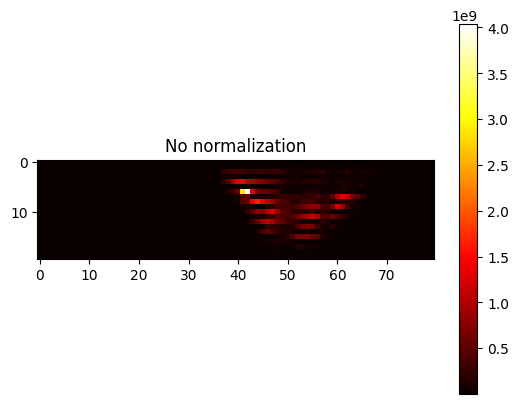
\includegraphics[width=.6\columnwidth]{images/sample_spectrogram.png}
    \caption{Spectrogram of a sample of the dataset}
    \label{fig-1}
\end{figure}
\section{Batch size selection}
Selecting an appropriate batch size is a critical factor in neural network training.
Opting for a higher value facilitates smoother convergence towards the minimum point;
however, each iteration becomes time-consuming as it needs to process a larger number of samples.
Conversely, a very low batch size can lead to unstable convergence, requiring more iterations.
On the positive side, each iteration is quicker since it processes only a limited number of samples.\newline
The figure below illustrates the test accuracy for different epochs and batch sizes in a model without hidden layers.
The model trained with a batch size of 10 exhibits gradual improvement but experiences oscillations.
Differently, the 200-sized batch demonstrates more consistent progress, albeit at a slower pace compared to the 50 and 100-sized batches.
Among these options, the 50-sized batch yields the highest accuracy, surpassing that of the 100-sized batch.
\begin{figure}[H]
    \centering
    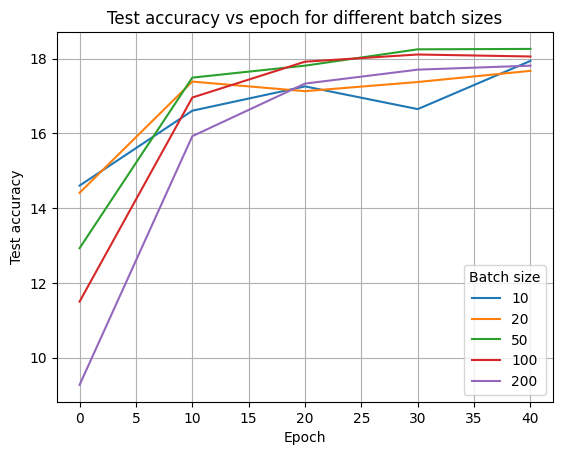
\includegraphics[width=.6\columnwidth]{images/batch_size.png}
    \caption{Test accuracy for different batch sizes}
    \label{fig-2}
\end{figure}

\pagestyle{OtherPage}
\section{Network architecture}
Numerous neural networks with varying depths and widths were trained to determine the optimal structure
and understand how performance is influenced by these characteristics. Evaluating the accuracy of training and
testing together is essential as the models can be susceptible to overfitting and underfitting. \\
Based on Figure \ref{fig-3}, it is evident that the network with 3 hidden layers and 1600, 512, 256, 128 and 35 neurons
respectively achieved the highest performance. Conversely, the network without hidden layers, consisting of only 1600 and 35 neurons,
performed poorly in comparison. \\
Furthermore, the figure demonstrates that increasing the depth of the network leads to improved training accuracy
while the test accuracy remains relatively unchanged, indicating a potential issue of overfitting.
This can be observed when transitioning from 2 to 3 hidden layers, where the model with 1600, 256, 128, 56 and 35 neurons
achieved significantly higher training accuracy than the model with 1600, 256, 128 and 35 neurons,
while their test accuracies were similar. The reason behind this discrepancy lies in the fact that increasing the depth of
the network enhances its flexibility, which may led to overfitting. \\
Conversely, when increasing the width of the network by augmenting the number of neurons per level, both training and
test accuracy improve proportionally. This occurs because such augmentation increases the complexity of the model without
necessarily enhancing its flexibility.

\begin{figure}[H]
    \centering
    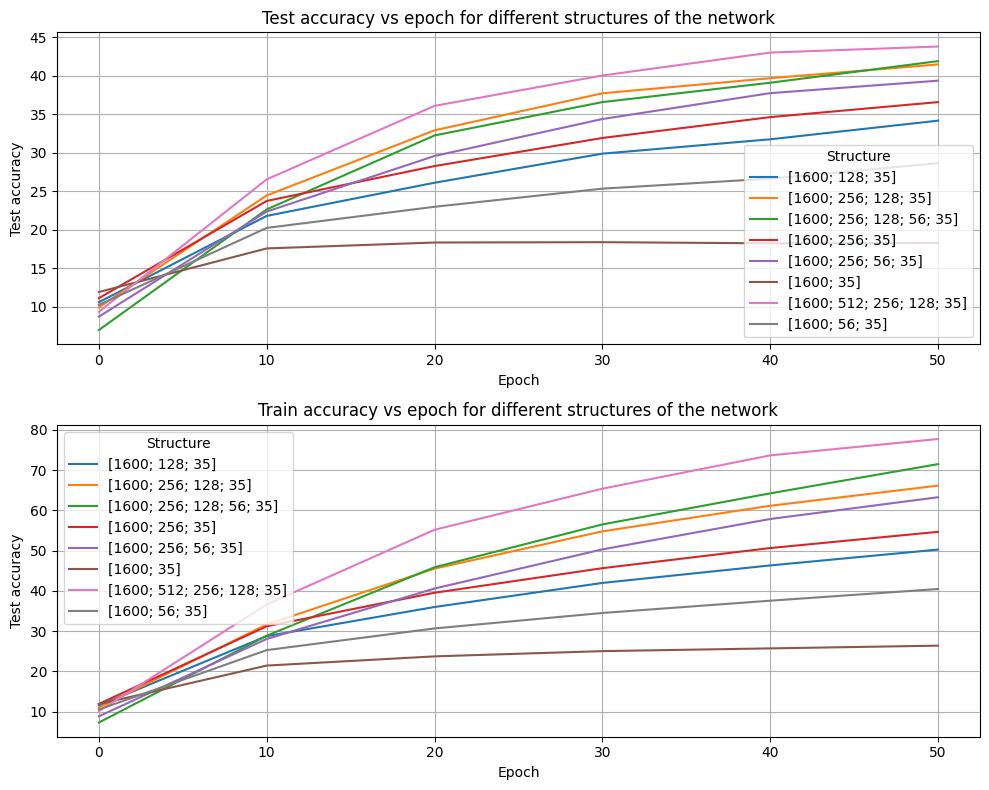
\includegraphics[width=\columnwidth]{images/diff_structures.png}
    \caption{Train and test accuracies for different network architectures}
    \label{fig-3}
\end{figure}

\subsection{Choice of the optimal lambda}

To mitigate overfitting, a regularization method can be employed, involving the addition of a regularization term to the neural network's cost function.
This term is calculated by squaring the network weights and multiplying them by a parameter lambda that governs its significance.
The process of determining the ideal lambda value involves testing various values, as depicted in Figure \ref{fig-4}.
The test accuracy indicates that the optimal lambda lies within the range of 0.0001 to 0.001, as these values yield higher accuracy on the test set.
\begin{figure}[H]
    \centering
    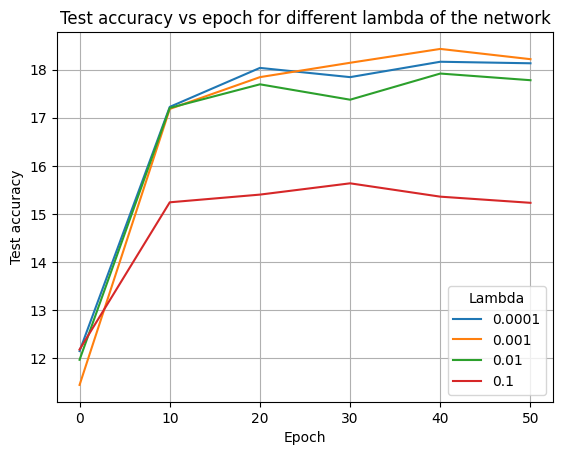
\includegraphics[width=.7\columnwidth]{images/lamda.png}
    \caption{Test accuracy for different lambda values}
    \label{fig-4}
\end{figure}

\subsection{Optimal network}
The optimal network architecture was found to be one with 3 hidden layers and 1600, 512, 256, 128, and 35 neurons, respectively.
The model was trained using previously obtained hyperparameters, which were a batch size of 50, a lambda value of 0.001, and 400 epochs.
The final test accuracy was measured at 0.4762, and the final training accuracy was found to be 0.8511.

\section{Model analysis}
The confusion matrix is a valuable method for analyzing model performance as it provides insights into how often a class (y-axis)
is incorrectly classified as another class (x-axis). To facilitate interpretation, the values in the matrix are expressed as percentages. \\
Figure \ref{fig-5} presents the confusion matrix, highlighting classes with the highest confusion rates.
Among the classes, the 'tree' class exhibits the poorest performance as it frequently gets misclassified as both 'two' and 'three'.
Following 'tree' is the 'forward' class, which often gets confused with 'follow' and 'four'.\\
To gain a deeper understanding of these classification errors, it is helpful to examine a sample of the words and analyze their corresponding spectrograms,
as depicted in Figure \ref*{fig-6}.
Upon inspection, it becomes evident that these misclassified words share similar acoustic characteristics and spectrogram patterns.
The model encounters difficulties in distinguishing these words due to their pronounced sound and spectrogram resemblances. \\
Furthermore, a comprehensive analysis revealed that the classes are imbalanced, with some classes having a large number of samples
while others have relatively few.
This class imbalance can impact the model's performance, as it tends to prioritize learning the well-represented classes while allocating
fewer resources to the underrepresented ones.
Consequently, classes with fewer samples exhibit lower accuracy, as illustrated in Figure \ref{fig-7}.
\begin{figure}[H]
    \centering
    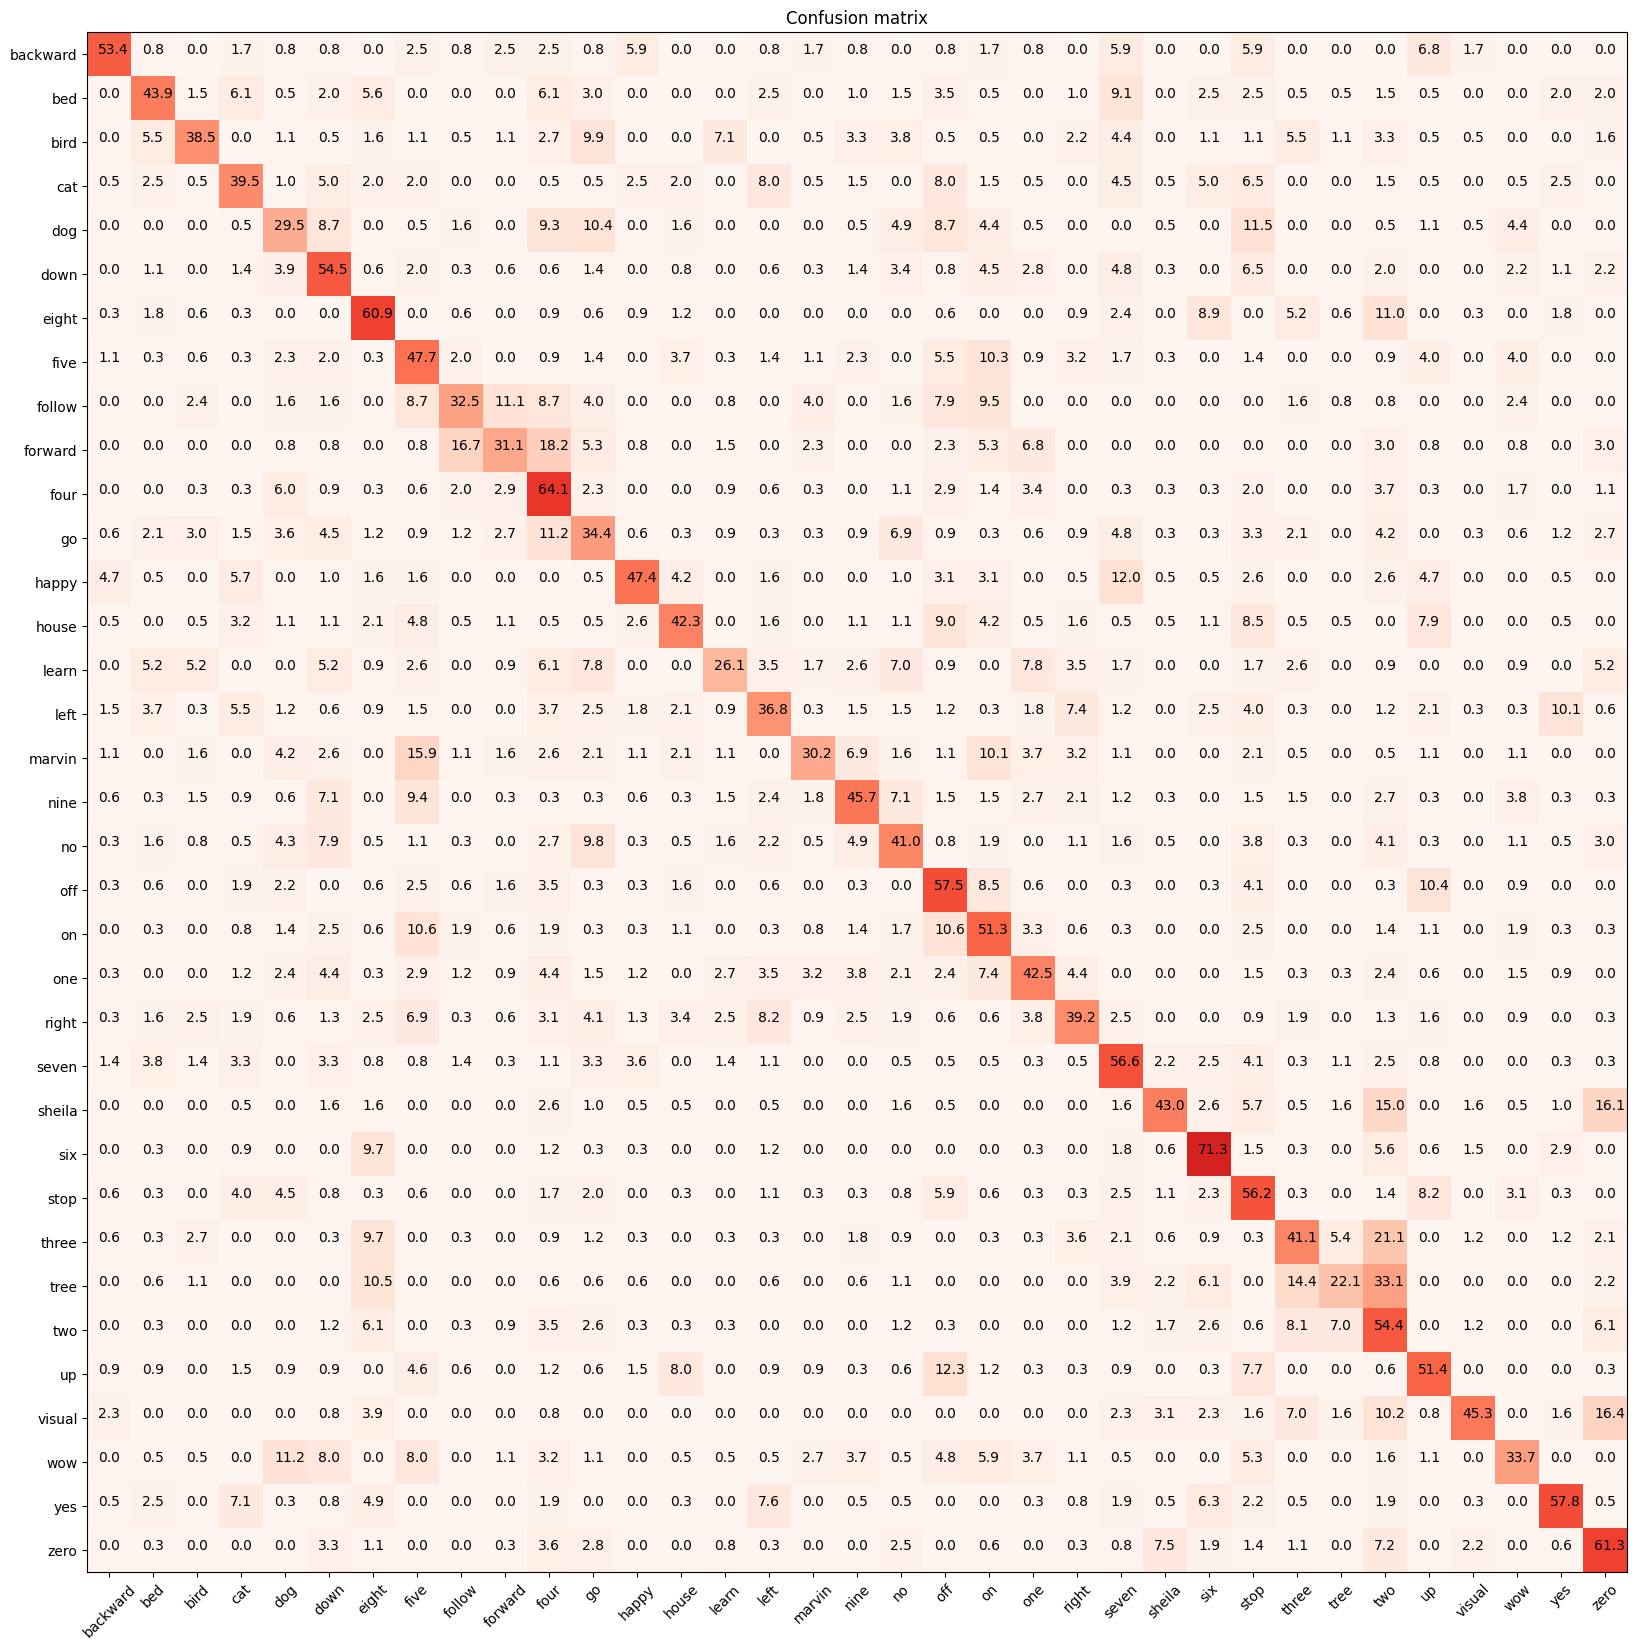
\includegraphics[width=\columnwidth]{images/confusion_matrix.png}
    \caption{Confusion matrix of the best model}
    \label{fig-5}
\end{figure}

\begin{figure}[H]
    \centering
    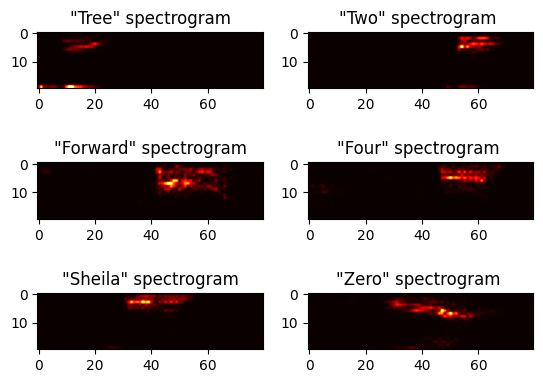
\includegraphics[width=.8\columnwidth]{images/misclassified_words.png}
    \caption{Spectrogram of the most 3 misclassified words, on left the correct word, on right the confused one}
    \label{fig-6}
\end{figure}

\begin{figure}[H]
    \centering
    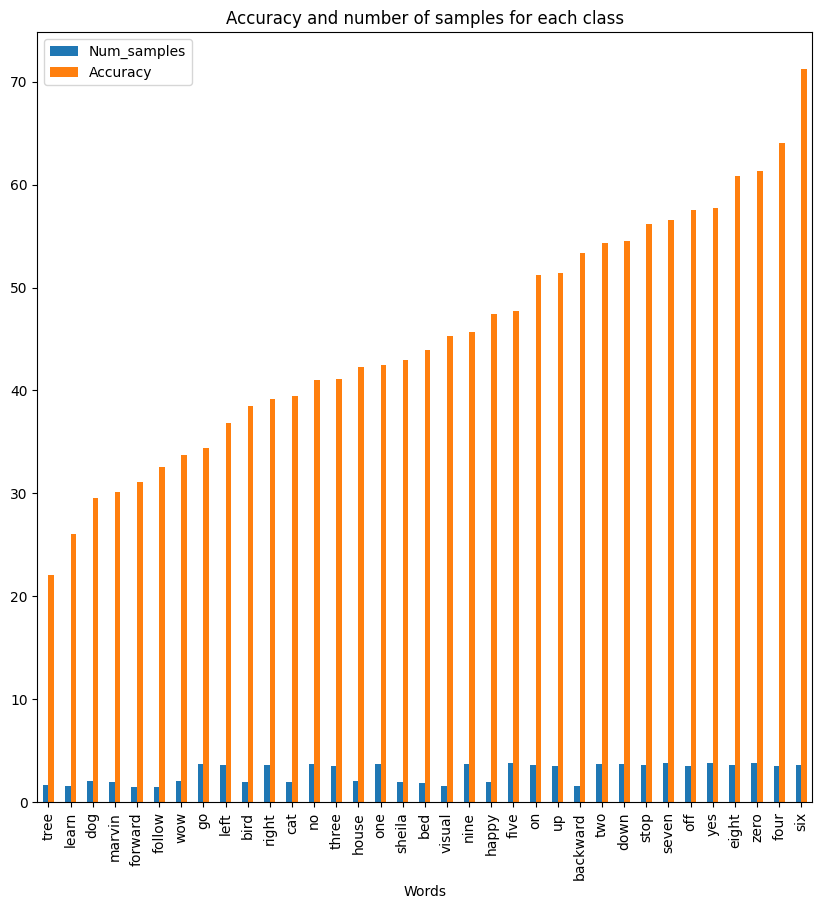
\includegraphics[width=.7\columnwidth]{images/num_vs_accuracy.png}
    \caption{Test accuracy and Number of samples (in percentage) for each class}
    \label{fig-7}
\end{figure}


\section{Feature normalization}
Normalization is a crucial preprocessing step that aims to enhance the performance of a model by transforming input variables. \\
Since the choice of the most suitable normalization technique may vary depending on the specific dataset and problem at hand,
in this project, the most common normalization methods were used: min-max scaling, mean-variance scaling, max absolute scaling and whitening.\\
The impact of these normalization methods on the input data can be visualized in Figure \ref{fig-8}, which displays the spectrogram of a sample from the dataset after applying each normalization technique. \\
To evaluate the effectiveness of these methods, the model was trained using the normalized data, and the corresponding accuracies are presented in Figure \ref{fig-9}.
By comparing the performance of the model trained with these normalization methods, it was observed that the mean-variance scaling method outperformed the others in terms of test accuracy.
\begin{figure}[H]
    \centering
    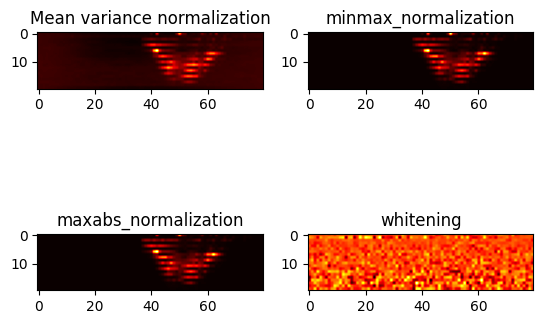
\includegraphics[width=.8\columnwidth]{images/normalization_spectrogram.png}
    \caption{Spectrogram of a sample of the dataset after different normalizations}
    \label{fig-8}
\end{figure}

\begin{figure}[H]
    \centering
    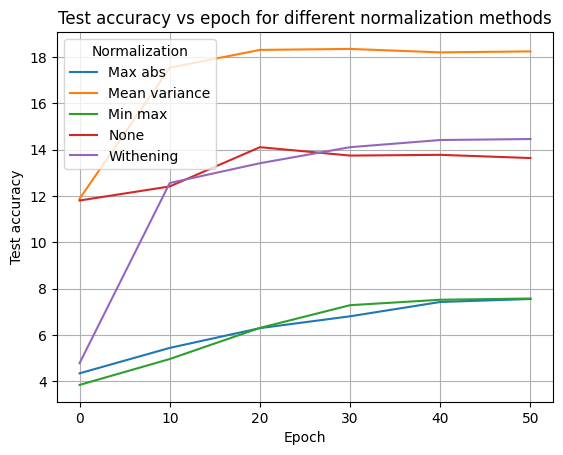
\includegraphics[width=.8\columnwidth]{images/test_diff_normalizations.png}
    \caption{Test accuracy for different normalizations}
    \label{fig-9}
\end{figure}
\section{Weights visualization}
The weights of the output layer were visualized by plotting their spectrogram, as depicted in Figure \ref{fig-10}.
In this visualization, the intensity of the weights is represented by colors, with red indicating high values and blue indicating low values. \\
By examining the figure, it becomes evident that the weights of the output layer bear resemblance to the spectrograms of the corresponding words they represent.
The visual alignment between the weight patterns and the spectrograms of the corresponding words supports the hypothesis that
the network has learned to extract relevant acoustic features and associate them with specific linguistic units. \\
Overall, the visualization of the output layer weights through spectrograms offers a valuable means of interpreting the neural network's
learned representations and verifying the effectiveness of the training process.

\begin{figure}[H]
    \centering
    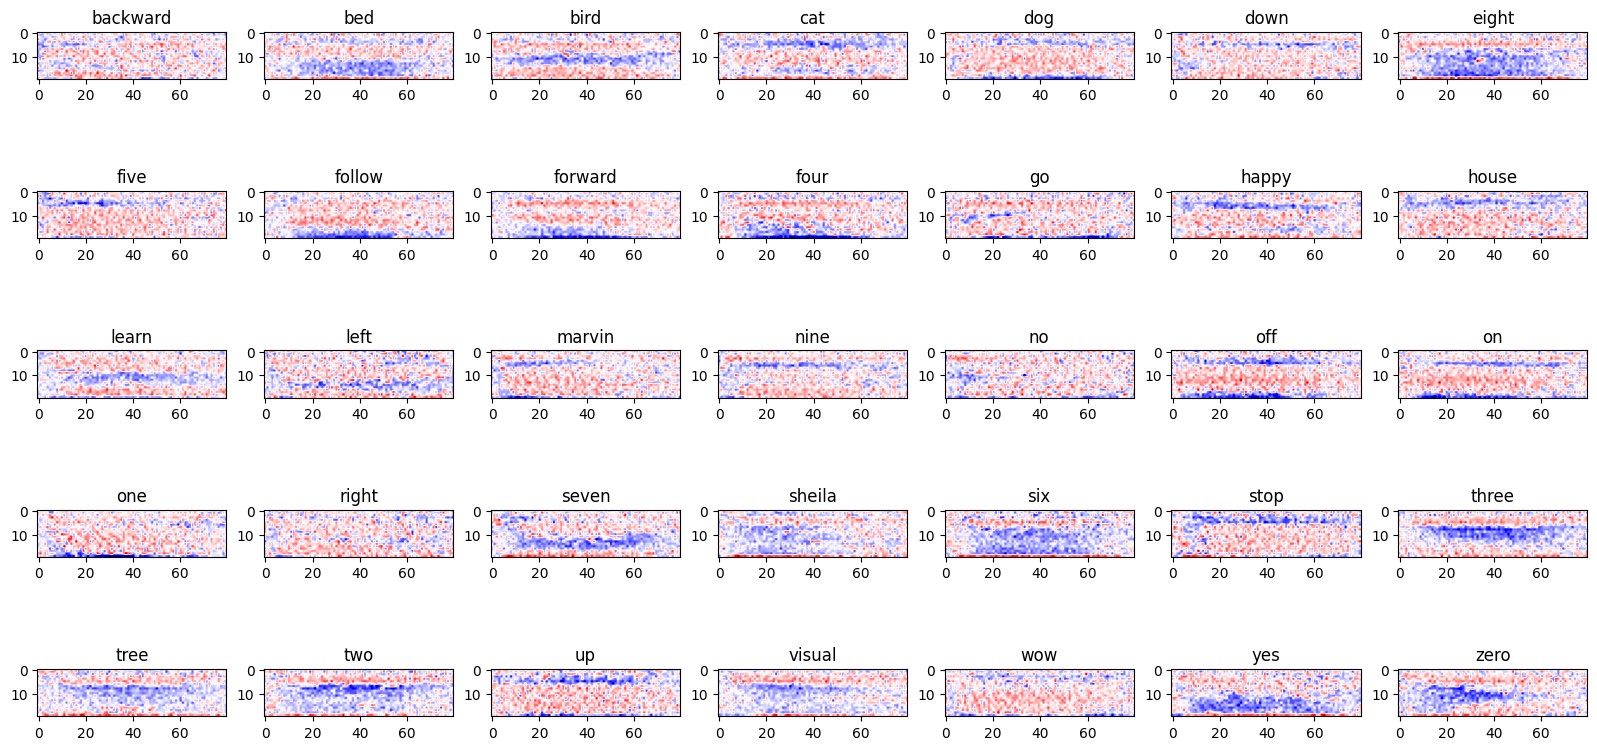
\includegraphics[width=\columnwidth]{images/spectrogram_weights.png}
    \caption{spectrogram of the weights of the output layer}
    \label{fig-10}
\end{figure}

\section{Declaration}
I affirm that this report is the result of my own work and that I did not share any part of it with anyone
else except the teacher.
\end{document}